\chapter{FLOCKING ALGORITHM}\label{chap3}

% introduction
%\section{Introduction}
The behavior seen in social animals like birds and fishes is called \textit{flocking}. Flocking algorithms are used to simulate this social behavior between entities by following a set of simple rules. These rules were introduced by the pioneer of flocking Craig Reynolds\cite{craig1}. The three main rules or steering behaviors are: separation, alignment, and cohesion. This chapter discuss the different behaviors implemented in our code, which include the three main steering behaviors, along with a three more.

% 3 steering behaviors
\section{Three Main Steering Behaviors}
The steering behaviors are velocity vectors, they have direction and magnitude. Each behavior is evaluated at each time step for each boid.

% separation
\subsection{Separation}\label{separationsection}
\textit{Separation} can be described as the steering force that maintains each entity of the flock separated by at least a minimum determined distance. Craig Reynolds first called this rule \textit{collision avoidance} because he was referring to avoid collision with nearby flockmates. Later on, the rule was named \textit{separation}. This steering behavior prevents the crowding between boids. Figure~\ref{separationPDF} shows that only flockmates within a certain radius are considered when evaluating this behavior. The red vector is the obtained steering force with this behavior.

% separation figure
\begin{figure}[htbp]
\begin{center}
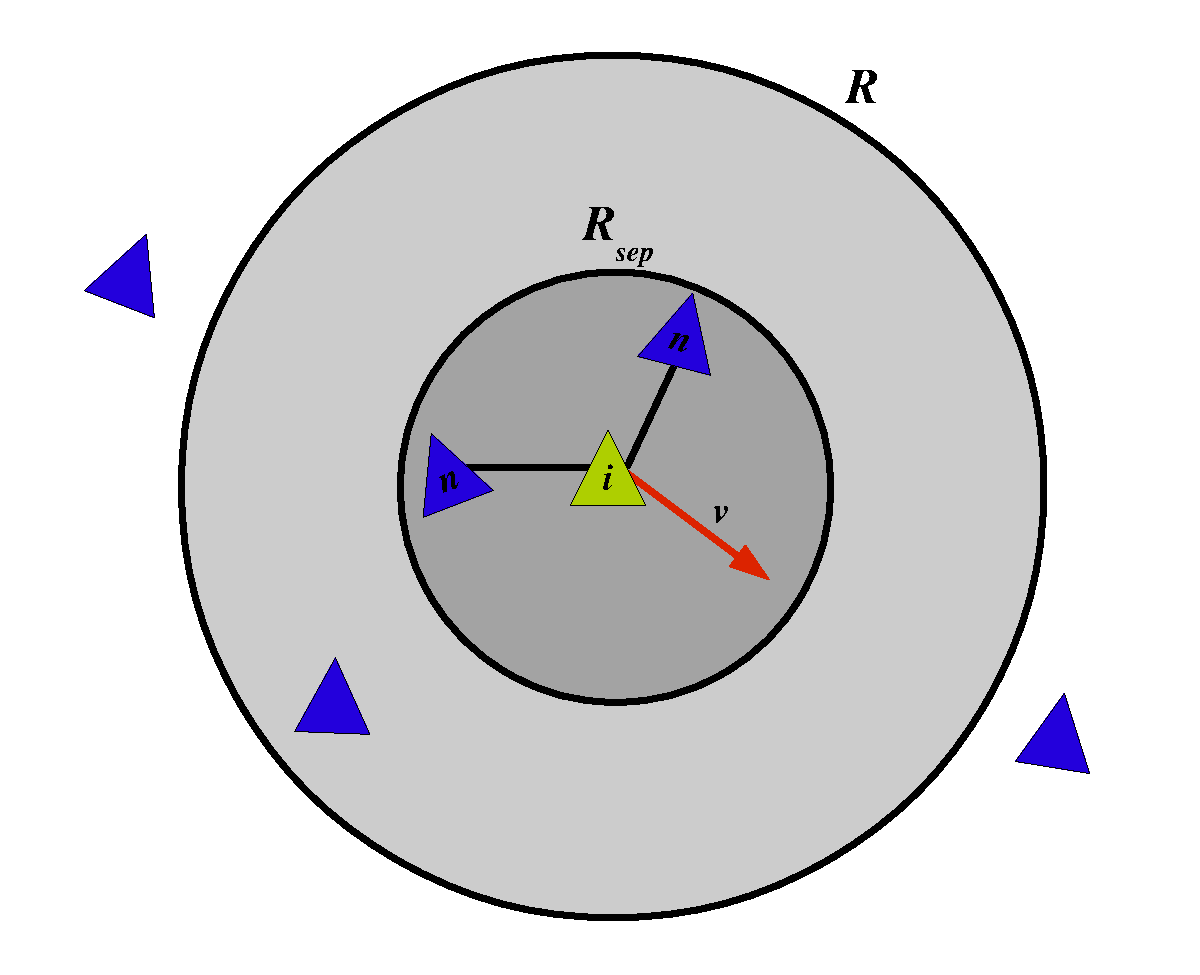
\includegraphics[scale=0.3]{figures/separation.pdf}
\caption{Separation steering force: the gray circle is the neighborhood of the green boid, \textit{separation} would steer the green boid away/near the neighboring boids until a minimum distance between them is met}
\label{separationPDF}
\end{center}
\end{figure}

Separation is a repulsive force. The mathematical expression that was implemented is showed in equation~\ref{separationEquation}.

% separation equation
\begin{equation}
\label{separationEquation}
Separation =\frac{1}{M} \sum_{n=1}^{M} \frac{p_i - p_n}{d(p_i,p_n)}
\end{equation}

Where $M$ is the number of boids within the minimum distance from the boid in question, $p_i$ is the position of boid $i$, and $d(p_i,p_n)$ is the distance between boids $i$ and boid $n$.

Only neighbors that are within the minimum separation distance are considered. The difference between the positions of boid $i$ and boid $n$ is divided by the distance between boid $i$ and boid $n$ are summed. Then, the sum is divided by the number of boids that were within the minimum distance. The resulting vector corresponds to the \textit{separation} steer of boid $i$ with respect to their nearest flockmates. 

% alignment
\subsection{Alignment}
\textit{Alignment} is the steering behavior that match the heading of all boids, and therefore aligning them to the same direction. Reynolds initially called this behavior \textit{velocity matching}, later the name was changed to \textit{alignment}. This behavior also prevents crowding along with \textit{separation}. As the name of the rule says, each boid would \textit{align} its heading with the average heading of their flockmates. Align with respect of direction and/or speed. Figure~\ref{alignmentPDF}  shows the corrective steering force vector in red.

% alignment figure
\begin{figure}[htbp]
\begin{center}
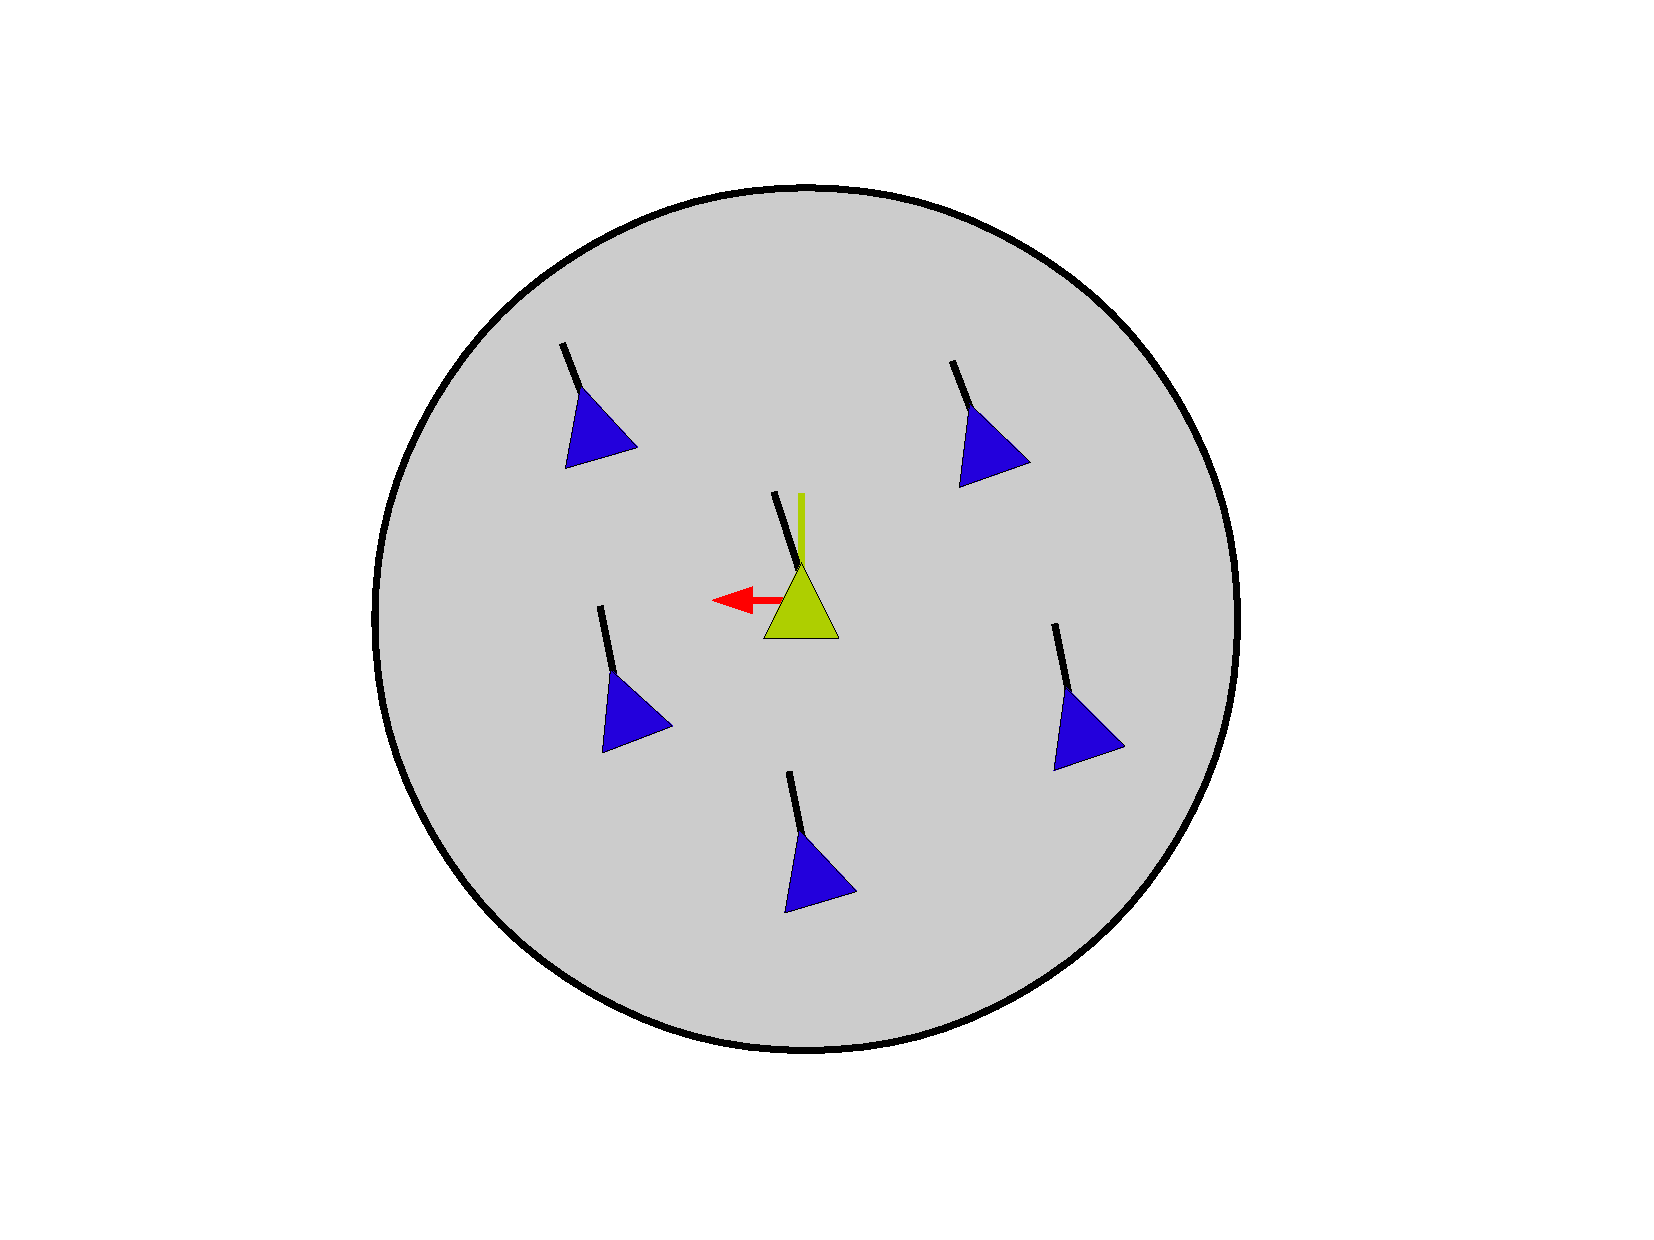
\includegraphics[scale=0.3]{figures/alignment.pdf}
\caption{Alignment steering force: the gray circle is the neighborhood of the green boid, \textit{alignment} match the heading and speed of the green boid with respect to the neighbors}
\label{alignmentPDF}
\end{center}
\end{figure}

\textit{Alignment} is also calculated in the local neighborhood of each boid. This steering behavior was computed using equation~\ref{alignmentEquation}.

% alignment equation
\begin{equation}
\label{alignmentEquation}
Alignment = \left[  \frac{1}{N} \sum_{n=1}^{N} v_n \right ] - v_i
\end{equation}

Where $N$ is the number of boids in the nearest neighbor within the search radius, this radius is bigger than the radius of the minimum separation distance used for \textit{separation}. $v_n$ is the velocity of boid $n$. The \textit{alignment} corrective force is computed by calculating the desired velocity which is the center of mass with respect to the velocities, and then subtracting the velocity of boid $i$ from it.

% cohesion
\subsection{Cohesion}
\textit{Cohesion} is the behavior that steers towards the center of the flock. When Reynolds introduced its \textit{Boids} model, he called this behavior \textit{flock centering} and defined it as \textit{the attempt to stay close to nearby objects}. The definition was kept while the name of the rule changed to \textit{cohesion}. This behavior makes each boid attracted to the center of the flock, in our case the calculation of the steering vector is using the local neighbor of each boid. The boids would be attracted to the center of mass of their local neighborhood.  Figure~\ref{cohesionPDF} shows the \textit{cohesion} steering force in red.

% cohesion figure
\begin{figure}[htbp]
\begin{center}
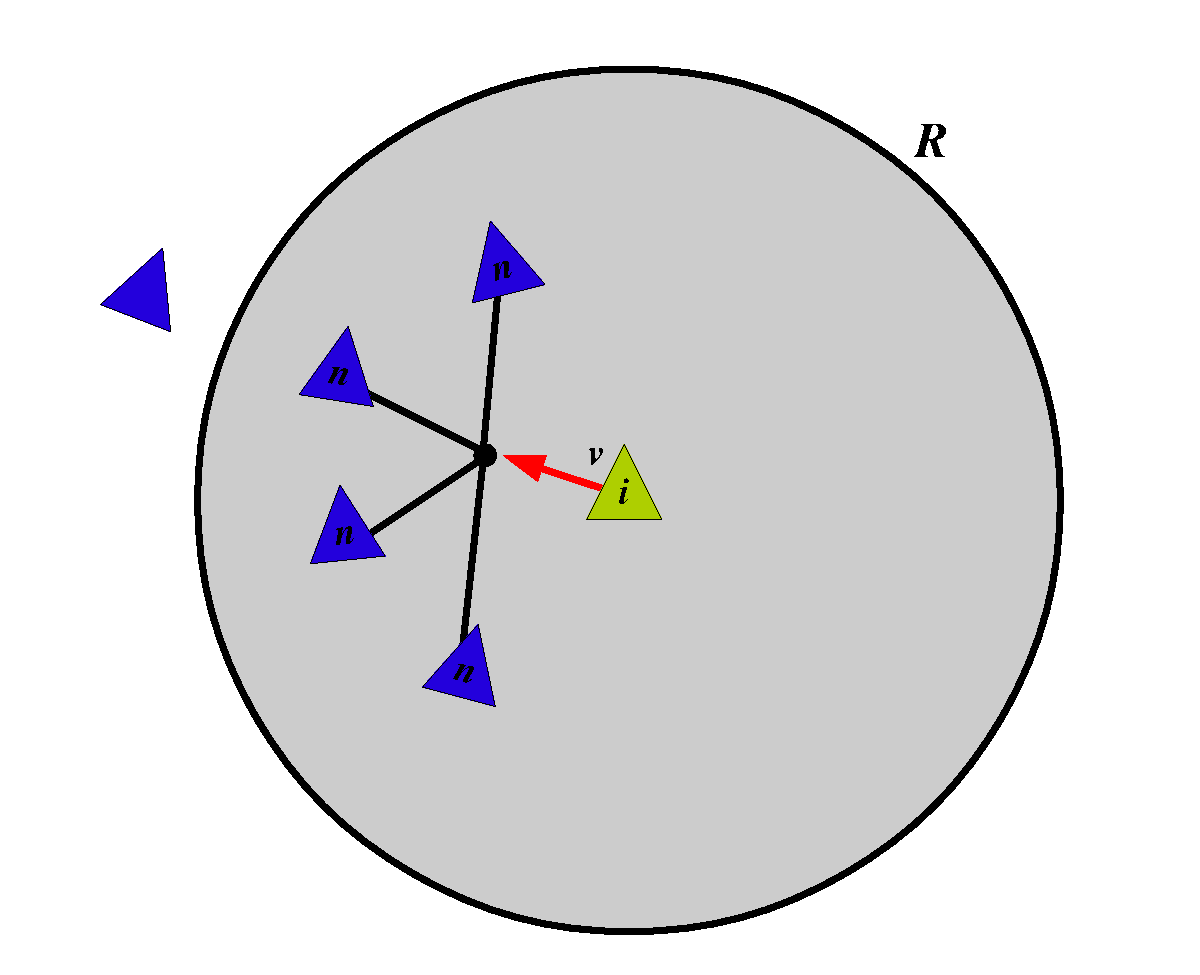
\includegraphics[scale=0.3]{figures/cohesion.pdf}
\caption{Cohesion steering force: the gray circle is the neighborhood of the green boid, \textit{cohesion} steers the green boid towards the center of their local neighborhood}
\label{cohesionPDF}
\end{center}
\end{figure}

The formula used for \textit{cohesion} is very similar to the formula used for \textit{alignment}, the only difference is that \textit{cohesion} uses the positions of the boids while \textit{alignment} uses the velocities of the boids. Equation~\ref{cohesionEquation} shows the \textit{cohesion} formula.

% cohesion equation
\begin{equation}
\label{cohesionEquation}
Cohesion = \left[  \frac{1}{N} \sum_{n=1}^{N} p_n \right ] - p_i
\end{equation}

Where $N$ is the number of boids in the local neighborhood of boid $i$. $p_n$ is the position of the flockmate $n$. The average position or center of mass is calculated using the flockmates of the local neighborhood, then the position of boid $i$ is subtracted from the average position. The resulting vector is the \textit{cohesion} steering force.

% other behaviors
\section{Other Steering Behaviors}\label{otherbehaviors}
Besides the three main steering behaviors discussed in the above Section many more steering forces have been formulated, see Section~\ref{currentwork} for a list of some of them. In this section only the behaviors that were implemented are discussed: \textit{goal}, \textit{avoid}, and \textit{follow the leader}.

% goal
\subsection{Goal}
\textit{Goal} is the steering behavior that attracts the boids to a specific location in global space. This location is static. Figure~\ref{seekfleePDF} shows the action taken when approaching or avoiding the target. The red vector shows the \textit{goal} steering, the blue vector, avoid, would be discussed in the next Section. The gray vector to the right of the boid is the desired velocity and the dotted line would be the path taken by the boid.

% seek and flee figure
\begin{figure}[htbp]
\begin{center}
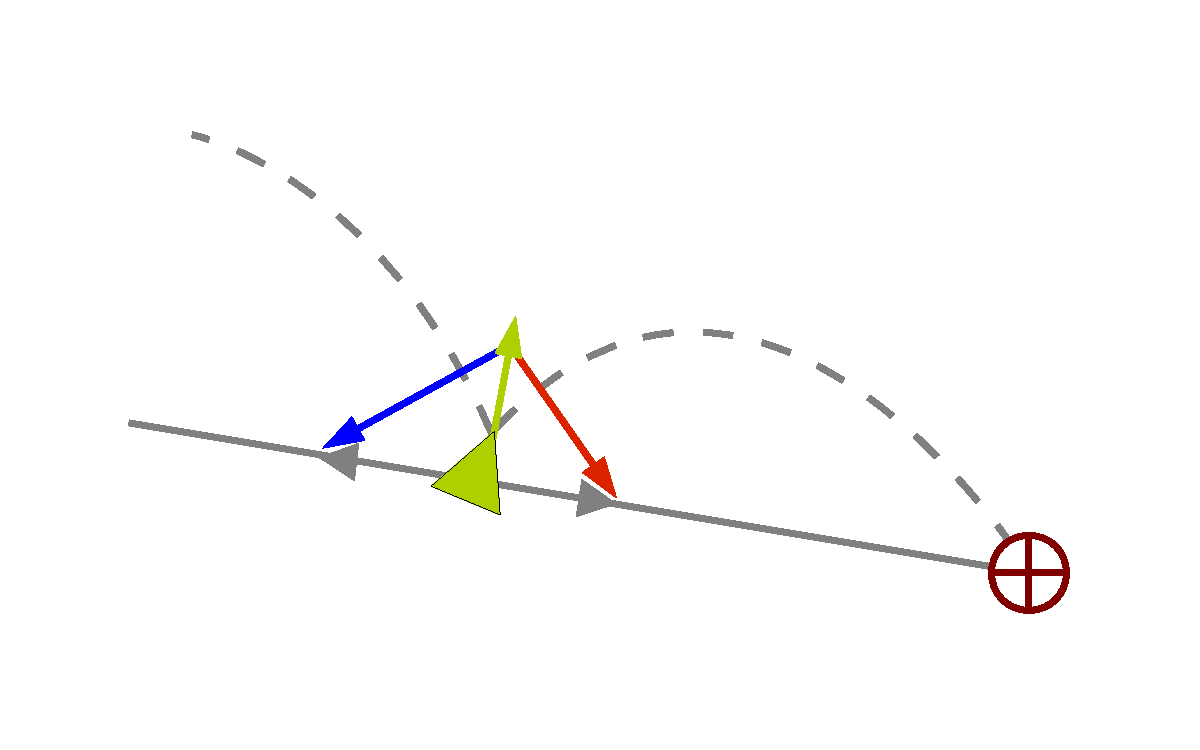
\includegraphics[scale=0.5]{figures/seekANDflee.pdf}
\caption{Goal and Avoid behaviors: the green boid would approach the target when is following the \textit{goal} behavior, or it would backing out from it when following the \textit{avoid} behavior }
\label{seekfleePDF}
\end{center}
\end{figure}

\textit{Goal} behavior adjusts the boid's velocity in a way that it is aligned towards the target. \textit{How it is computed?} Since the target is static, the position of the boid is subtracted from the position of the target, the resulting vector is normalized and multiplied by the maximum speed of the boid. This vector is the desired velocity at which the boid is going to steer. To get the steering vector, subtract the current velocity vector from the desired velocity vector. The implemented formula is in equation~\ref{goalEquation}

% goal equation
\begin{equation}
\label{goalEquation}
Goal = ((p_t - p_i) * max_{speed}) - v_i
\end{equation}

Where $p_i$ and $v_i$ are the position and velocity of boid $i$, respectively. This rule causes the boid to keep approaching the goal over and over, kind of like moth buzzing around a light bulb.

% avoid
\subsection{Avoid}
\textit{Avoid} means to steer away from a static target in the global space. The approach is similar to to the \textit{goal} steering with a difference in that the desired velocity will be pointing to the opposite direction. Figure~\ref{seekfleePDF} depicts the steering vector in blue and the desired velocity in gray (at the left side of the boid). Notice that the desire velocity vector for both \textit{goal} and \textit{avoid} are pointing in opposite directions. Equation~\ref{avoidEquation} shows the mathematical formula for \textit{avoid}.

% avoid equation
\begin{equation}
\label{avoidEquation}
Avoid = -((p_t - p_i) * max_{speed}) - v_i
\end{equation}

$((p_t - p_i) * max_{speed})$ is called the desired velocity. For the \textit{avoid} behavior there is a negative sign preceding the desired velocity, therefore it would be pointing to the opposite direction of the desired velocity for the \textit{goal} behavior.

% leader following
\subsection{Follow the Leader}
The \textit{Follow the Leader} behavior is when there is a boid in charge of the flock, called \textit{leader}, and the rest of the boids in the flock the \textit{followers} follow him. This is one of the many complex behaviors that a flock can exhibit as a whole. Followers come after a point slightly behind the leader, its target while the leader approaches randomly selected locations as its target.

% leader following figure
\begin{figure}[htbp]
\begin{center}
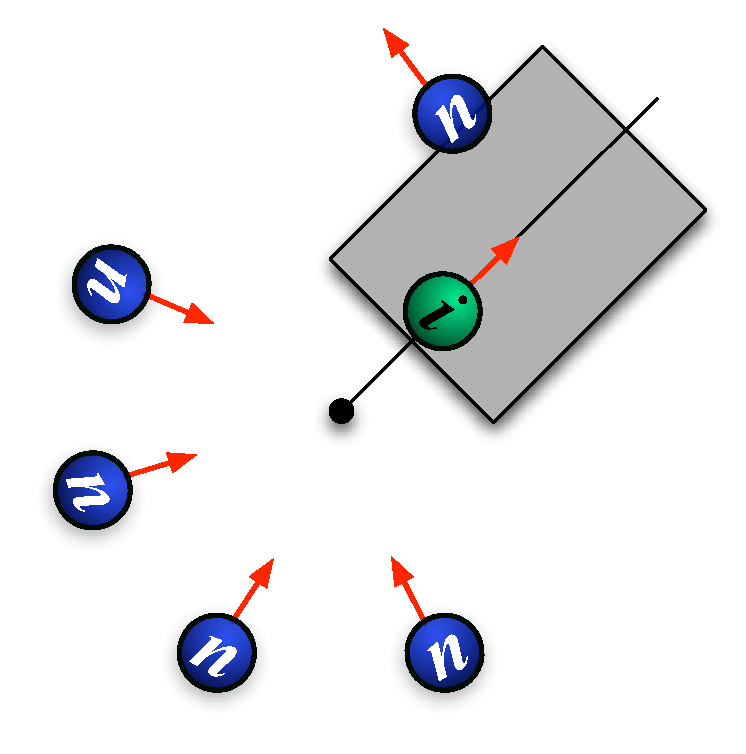
\includegraphics[scale=0.5]{figures/leaderFollowing.pdf}
\caption{Leader Following behavior: the followers would follow the leader by approaching a point slightly behind the leader, if a follower find itself in a rectangular area in front of the leader it would move out of the way of the leader}
\label{leaderPDF}
\end{center}
\end{figure}

Most of the time the followers want to stay closer to the leader without getting into its way. As can be seen in Figure~\ref{leaderPDF}.  If a follower is inside the rectangular region in front of the leader it moves away from it, leaving clear the way of the leader to move freely without worrying about colliding with their flockmates. The leader computes its movement using Equation~\ref{goalEquation} where $p_t$ is a random position within the global space. The followers that are outside the rectangular region will approach a point slightly behind from the leader using also Equation~\ref{goalEquation}.

% combining behaviors
\section{Combining the Steering Behaviors}
Each of the steering behaviors discussed above would return a velocity vector. Now the question arise on \textit{how to combine the behaviors in order to move the boids?}. Each steering force multiplied by a respective weight\footnote{Weights are given by the user, they are not constant values assigned by us.}. For example, combining \textit{separation}, \textit{alignment}, and \textit{cohesion} is done by using Equation~\ref{combine}. Each behavior is multiplied by its constant weight, then they are added to get the final velocity vector.

% combine equation
\begin{equation}
\label{combine}
velocity = C_S Separation  + C_A Alignment  + C_C Cohesion 
\end{equation}

The \textit{new} velocity is just the velocity of Equation~\ref{combine} plus the current velocity. Then, first order Euler integration method is used  to calculate the \textit{new} position of each boid. As shown in Equation~\ref{integrate}, where $p_i^{k+1}$ is the position of boid $i$ at step $k+1$, $v_i$ is the velocity of the boid, and $dt$ is the time step of the integration.

% integrate equation
\begin{align}
\label{integrate}
p_i^{k=1} = p_i^k + dt~ v_i
\end{align}

Each of the steering behaviors is calculated and combined for each boid every time step in order to update their positions.

% algorithms
\section{Algorithms}

In this Section three algorithms are going to be presented. The first one is the algorithm developed to compute the different rules implemented. The second one is the algorithm that combines the rules and compute the new positions of the boids. The last algorithm presented is the algorithm used to update all the boids at each frame of the simulation. 


The following Algorithm presents how we computed each of the rules on the GPU. Not all rules are computed at once, only rules with weights greater than zero would be computed.

% flocking algorithm
\begin{algorithm}
\caption{Flocking algorithm to follow Separation, Alignment, Cohesion, Goal, and Avoid steering behaviors}
\label{flockingAlgorithm}
\begin{algorithmic}
\FOR {each neighbor $j$ of boid $i$}
	\IF{dist($i$, $j$) $<=$ searching radius}
	\STATE flockmates++
		\IF{$w_{sep} > 0$}
			\IF{dist($i$, $j$) $<=$ minimum distance}
				\STATE nearestFlockmates++
				\STATE s = $pos_i$ - $pos_j$ 
				\STATE s /= dist($i$, $j$) 
				\STATE separation += s
			\ENDIF
		\ENDIF
		\IF{$w_{align} > 0$}
			\STATE alignment += velocity($j$)
		\ENDIF
		\IF{$w_{coh} > 0$}
			\STATE cohesion += position($j$)
		\ENDIF
	\ENDIF
\ENDFOR
\IF{$w_{sep} > 0$ \&\& nearestFlockmates $> 0$}
	\STATE separation /= nearestFlockmates
\ENDIF
\IF{$w_{align} > 0$ \&\& flockmates $> 0$}
	\STATE alignment /=  flockmates
	\STATE alignment -= velocity($i$)
\ENDIF
\IF{$w_{coh} > 0$ \&\& flockmates $> 0$}
	\STATE cohesiont /=  flockmates
	\STATE cohesion -= position($i$)
\ENDIF
\IF{$w_{goal} > 0$}
	\STATE $pos_t$ = target
	\STATE desiredVel = normalize($pos_t - pos_i$) * $max_{speed}$
	\STATE goal = desiredVel - $vel_i$
\ENDIF
\IF{$w_{avoid} > 0$}
	\STATE $pos_t$ = target
	\STATE desiredVel = -normalize($pos_t - pos_i$) * $max_{speed}$
	\STATE avoid = desiredVel - $vel_i$
\ENDIF

\end{algorithmic}
\end{algorithm}

What is cleaver about Algorithm~\ref{flockingAlgorithm} is that each of the rules is computed independently, not all at once. Algorithm~\ref{flockingAlgorithm} has various steps. Note that the iterative loop is over the flockmates of boid $i$. First we count how many flockmates are in the neighborhood determined by a searching radius. The number of flockmates is needed for the rules \textit{cohesion} and \textit{alignment}. Then, if the weight of the rule is greater than zero, that rule is computed. Since we do not want to waste computations by computing rules that the user do not want to use. The steering vectors that store the values for the rules are initialized with zeros and there is no problem if the rule is not calculated since when combining them, there is going to be no error in the computation of the final velocity vector.

An similar approach was taken for the CPU implementation of Algorithm~\ref{flockingAlgorithm}.

% combine and integrate
\begin{algorithm}
\caption{Combine the steering vectors, calculate new position and check the boundaries}
\label{combineAlgorithm}
\begin{algorithmic}
\STATE Multiply each steering behavior by its respective weight to get the weighted velocity.
\STATE Combine the weighted velocities by adding them to get the final velocity.
\STATE Constraint the final velocity to a maximum allowed speed.
\STATE Integrate over time to get the new position.
\STATE Apply periodic boundary conditions to the new position.
\end{algorithmic}
\end{algorithm}

Algorithm~\ref{combineAlgorithm} presents the steps done to calculate the new position of each boid at each time step.

% update
\begin{algorithm}
\caption{Update of each frame of the simulation}
\label{updateAlgorithm}
\begin{algorithmic}
\STATE Create a FLOCK particle system.
\FOR {each frame}
\STATE Do the nearest neighbor search.
\STATE Compute that rule.
\STATE Integrate over time.
\STATE Render the new position.
\ENDFOR
\end{algorithmic}
\end{algorithm}

The Algorithm~\ref{updateAlgorithm} is a simplify version of what the \texttt{updateGPU()} function does. See Section~\ref{flocksection} for more details of the \texttt{updateGPU()} function. First a FLOCK system has to be created then the boids enter into a loop that is going to be running until the user quits the simulation.

